\documentclass[10pt]{article}
\usepackage{setup}
\usepackage[framed,numbered,autolinebreaks,useliterate]{mcode}
\vspace{-8ex}
\date{}

\graphicspath{{../figs/}}

\begin{document}

\title{\textbf{\Large{\textsc{ECE446:} Sensory Communication}} \\ \Large{Digital Signal Processing Problem Set Report}\vspace{-0.3cm}}
\author{Pranshu Malik\\ \footnotesize{1004138916}\vspace{-3cm}}

\maketitle

\section{Manipulation of Signals in the Frequency Domain}
Matches $\hat{x}(t) = \cos(2\pi440t) - \sin(2\pi660t)$ sampled at $t = nT_s$, i.e. $\hat{x}[n] \coloneqq \hat{x}(nT_s)$. By a similar transformation, we can recover the time-domain equaivalent of the signal, showing as scaled deltas. This is one part of the internals in \texttt{sound} function in matlab. The sound can be played here: give github repo/online host.

\begin{figure}[ht]
    \centering
    \begin{subfigure}[b]{0.48\textwidth}
        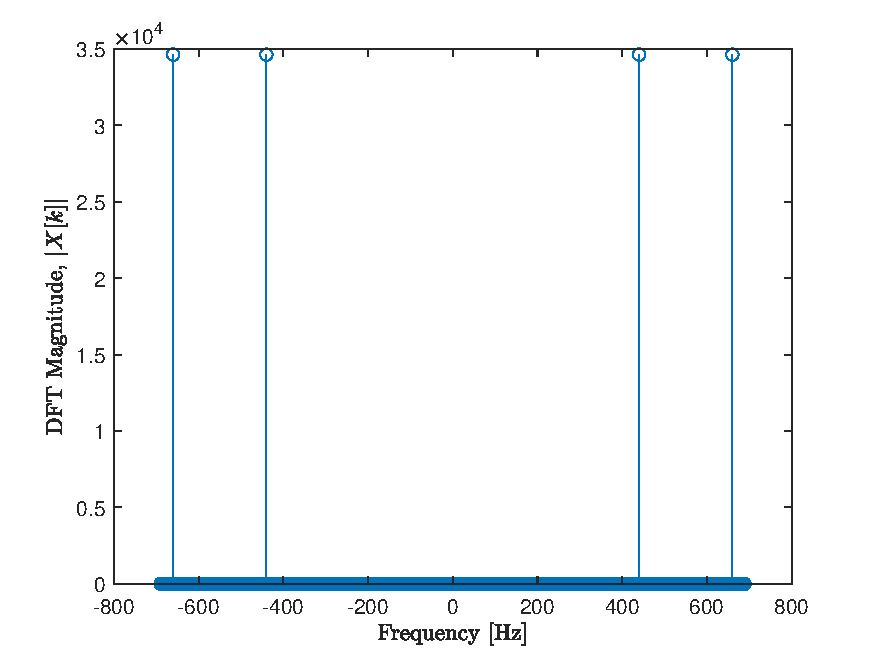
\includegraphics[width=\textwidth]{problem1_fft.pdf}
        % \caption{}
    \end{subfigure}
    \quad
    \begin{subfigure}[b]{0.48\textwidth}
        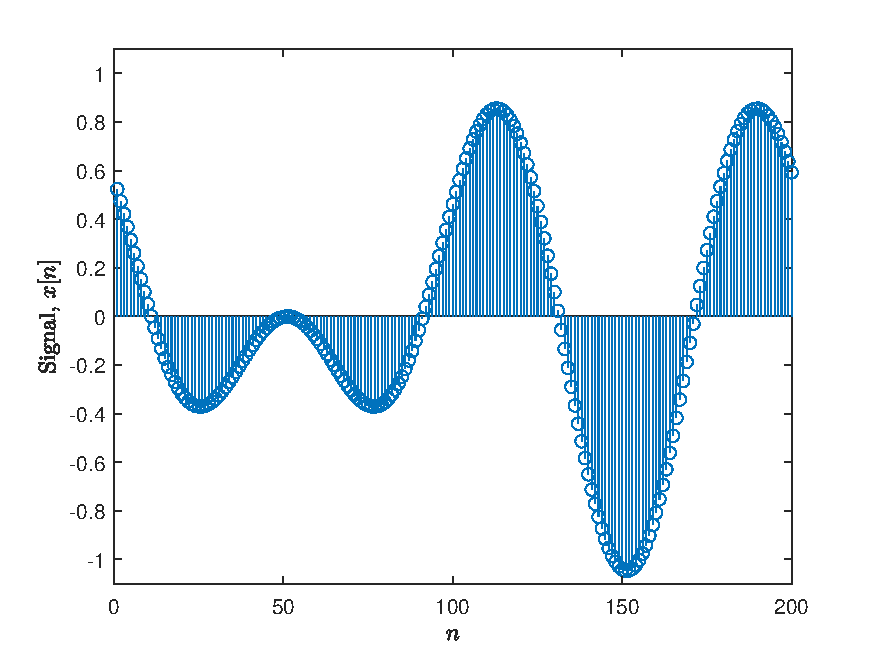
\includegraphics[width=\textwidth]{problem1_sig.pdf}
        % \caption{}
    \end{subfigure}
    \caption{Signals nice ones <>\vspace{-0.5cm}}
    \label{freq_domain_design_for_time_domain_signal}
\end{figure}

More text here.

\section{Effect of Time Windowing on the Frequency Spectra}

Done. Some explanation. See \ref{time_bandwidth_tradeoff} for more info. THough notice, that there is no visible deviation from the true frequency, however if samples (and hence sampling duration) were low enough, we would see a distortion in the freq spectrum due to overlapping/conv with rect....

\begin{figure}[ht]
    \centering
    \begin{subfigure}[b]{0.48\textwidth}
        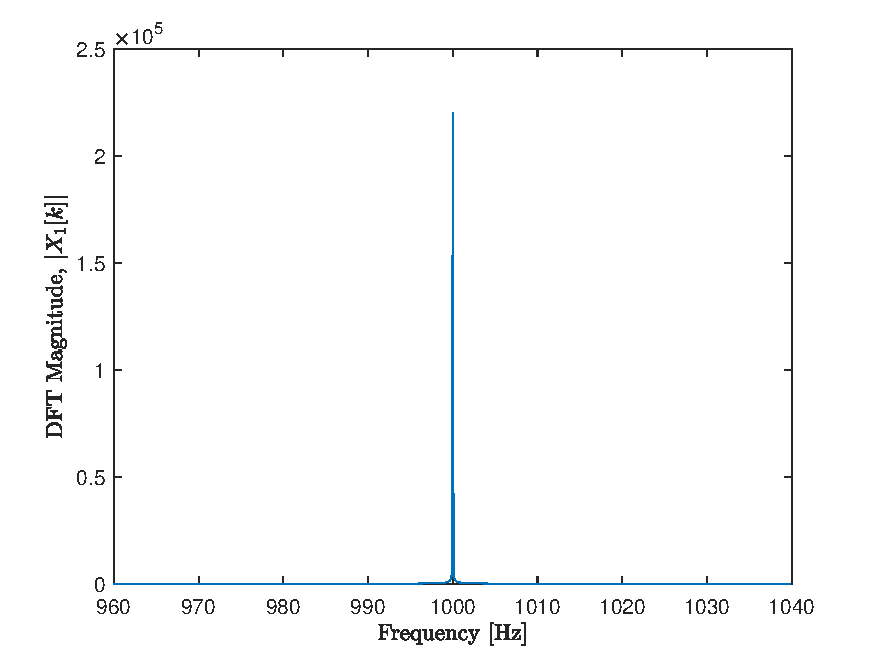
\includegraphics[width=\textwidth]{problem2_fft_high_dur.pdf}
        \caption{High Dur}
    \end{subfigure}
    \quad
    \begin{subfigure}[b]{0.48\textwidth}
        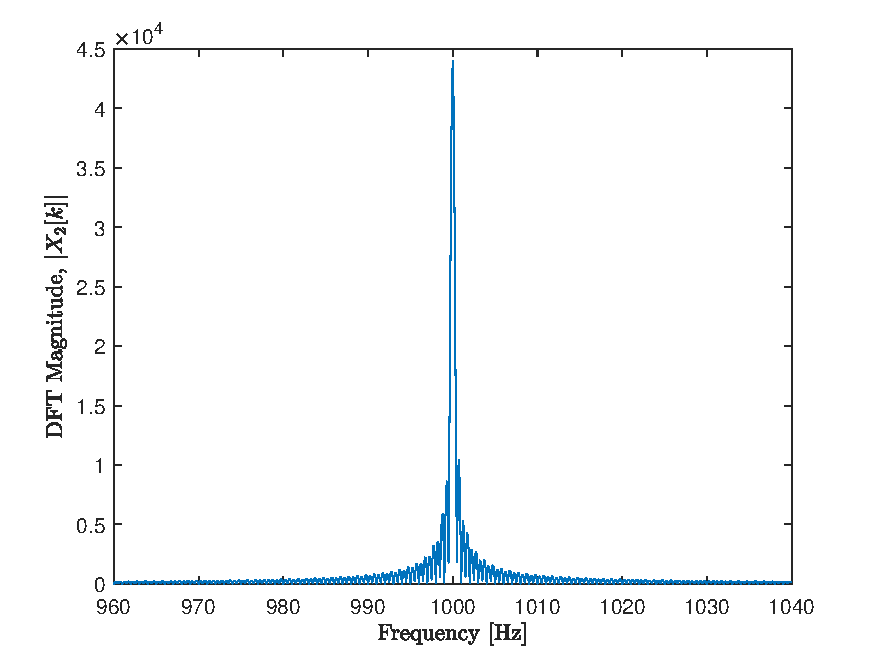
\includegraphics[width=\textwidth]{problem2_fft_low_dur.pdf}
        \caption{Low Dur}
    \end{subfigure}
    \caption{Effect of dur of FFT <>\vspace{-0.5cm}}
    \label{time_bandwidth_tradeoff}
\end{figure}

\section{Telephone Dial Tones}
Done. The dialtone signals were generated using the given $f_\text{low}$ and $f_\text{high}$. mention the freq combinations for dialtones 1, 2, and 4.
\[
    0.5*(cos(2*pi*fl1*t) + cos(2*pi*fu1*t));
\]

\section{Dial Tone Decode Algorithm}
Done. In real life, this can also be done using an analog circuit, with parallel and tuned filters with mediocre $Q$ to make them robust to noise on the channel, hence our decision to include an $\epsilon -$frequency band (\texttt{fr\_eps} in code) for robustness to noise and distortion.

The algorithm is as follows:
\begin{figure}[ht]
  \centering
  \begin{minipage}{.5\linewidth}
        \begin{algorithm}[H]
            \caption{An algorithm with caption}\label{alg:cap}
            \begin{algorithmic}
                \Require $n \geq 0$
                \Ensure $y = x^n$
                \State $y \gets 1$
                \State $X \gets x$
                \State $N \gets n$
                \While{$N \neq 0$}
                \If{$N$ is even}
                    \State $X \gets X \times X$
                    \State $N \gets \frac{N}{2}$  \Comment{This is a comment}
                \ElsIf{$N$ is odd}
                    \State $y \gets y \times X$
                    \State $N \gets N - 1$
                \EndIf
                \EndWhile
            \end{algorithmic}
        \end{algorithm}
    \end{minipage}
\end{figure}

The \textsc{MATLAB} code can be found in the appendix.

\section{Telephone Event Tones}
Done. The telephone event tones were generated in a similar fashion to problem 3. Check the dsp script for the code.

\section{Helmholtz Resonators}
Done. $\omega = c\sqrt{\frac{S}{V_0l}}$. Did about 1/3 bottle as getting 1/2 to resonante was very hard for the type of bottle. $153.4\sqrt{\frac{3}{2}} = 187.87 \approx 190.7$.

\begin{figure}[ht]
    \centering
    \begin{subfigure}[b]{0.48\textwidth}
        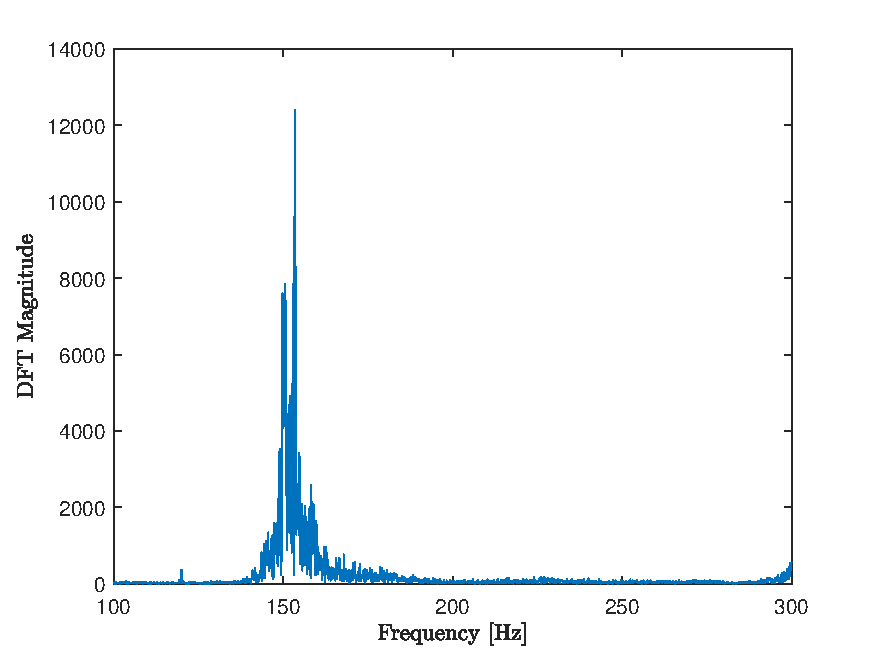
\includegraphics[width=\textwidth]{problem6_empty_bottle_resonance_spectra.pdf}
        \caption{High Dur}
    \end{subfigure}
    \quad
    \begin{subfigure}[b]{0.48\textwidth}
        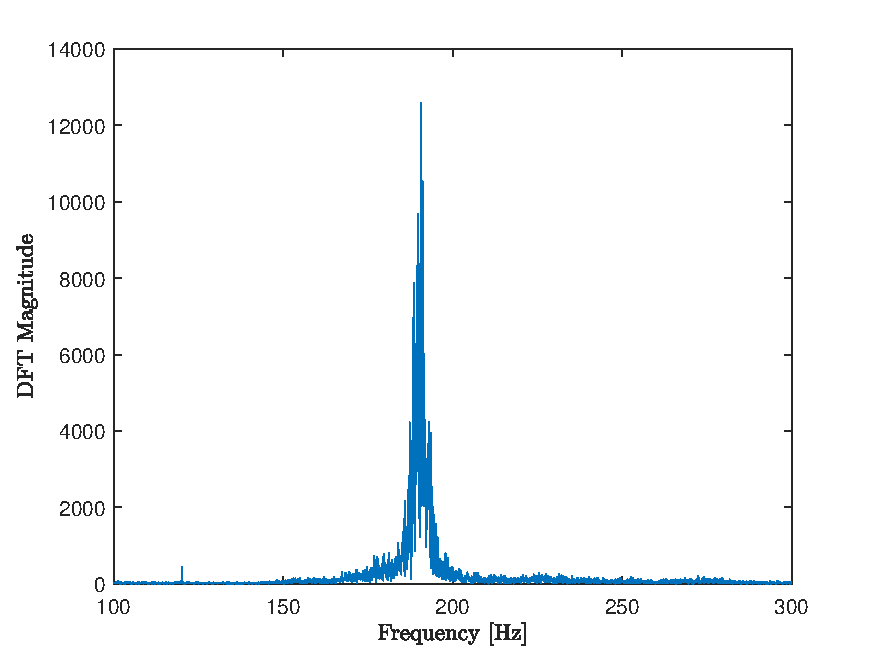
\includegraphics[width=\textwidth]{problem6_filled_bottle_resonance_spectra.pdf}
        \caption{Low Dur}
    \end{subfigure}
    \quad
    \begin{subfigure}[b]{0.48\textwidth}
        \centering
        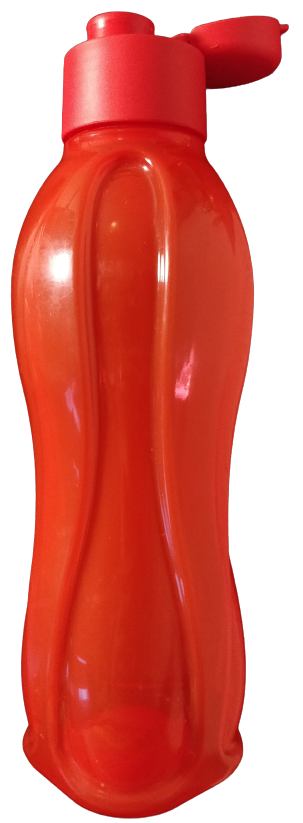
\includegraphics[scale=0.15]{bottle.png}
        \caption{Low Dur}
    \end{subfigure}
    \caption{Helmholtz Resonance on A bottle\vspace{-0.5cm}}
    \label{helmholtz_resonance}
\end{figure}

\section{Comparison of Voice and Instrument Timbre}
Violin has 440 as the fundamental harmonic and has 2 sub harmonics and all above; structure to the spread. Voice has two main harmonics 440 and 220 and they reduce in magnitude, without much "structure". Shows different timbre (or lack of, thereof).

\begin{figure}[ht]
    \centering
    \begin{subfigure}[b]{0.48\textwidth}
        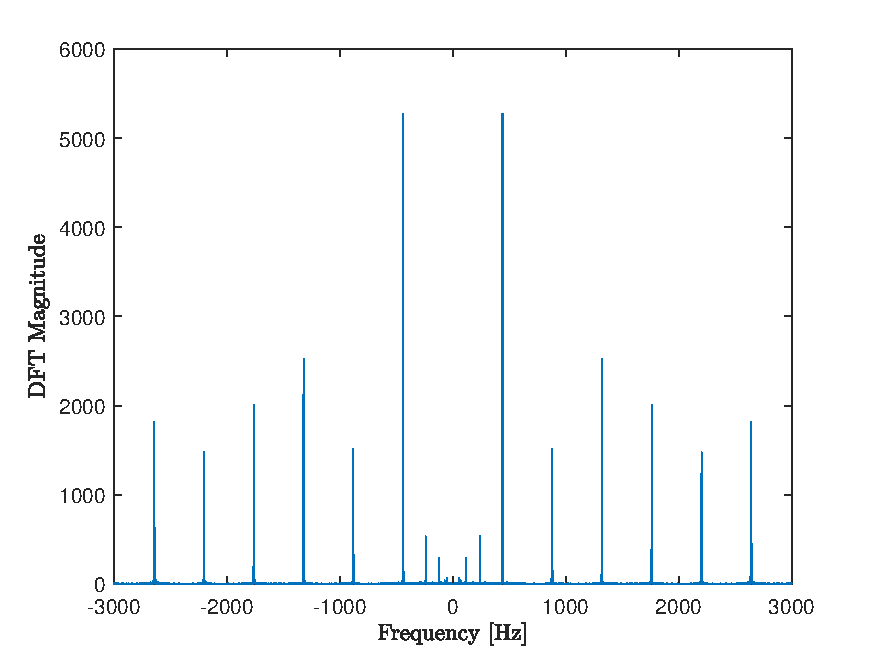
\includegraphics[width=\textwidth]{problem7_a440_violin_spectra.pdf}
        \caption{High Dur}
    \end{subfigure}
    \quad
    \begin{subfigure}[b]{0.48\textwidth}
        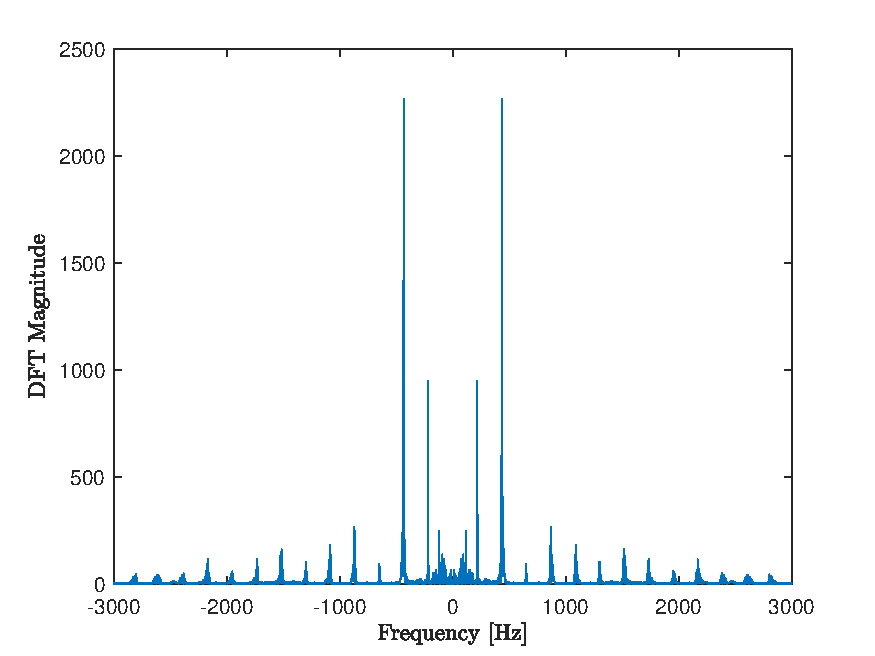
\includegraphics[width=\textwidth]{problem7_a440_voice_spectra.pdf}
        \caption{Low Dur}
    \end{subfigure}
    \quad
    \begin{subfigure}[b]{0.48\textwidth}
        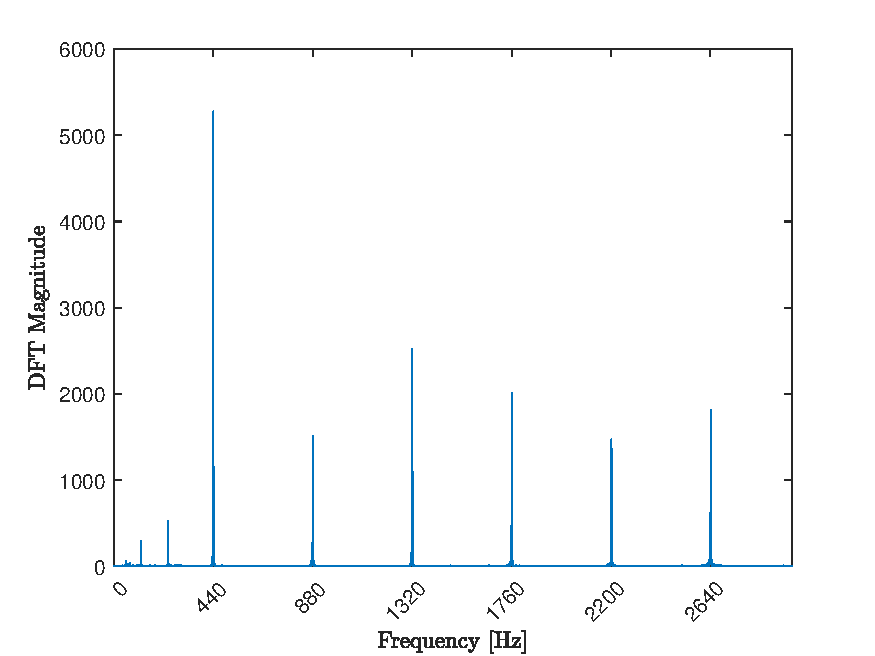
\includegraphics[width=\textwidth]{problem7_a440_violin_harmonics.pdf}
        \caption{Violin Harmonics}
    \end{subfigure}
    \quad
    \begin{subfigure}[b]{0.48\textwidth}
        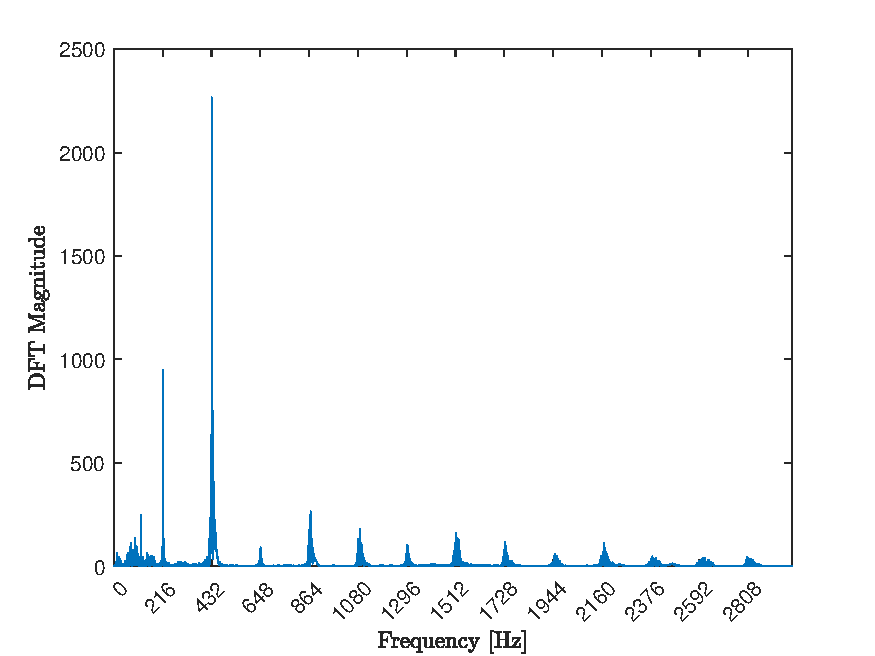
\includegraphics[width=\textwidth]{problem7_a440_voice_harmonics.pdf}
        \caption{Low Dur}
    \end{subfigure}
    % \quad
    % \begin{subfigure}[b]{0.48\textwidth}
    %     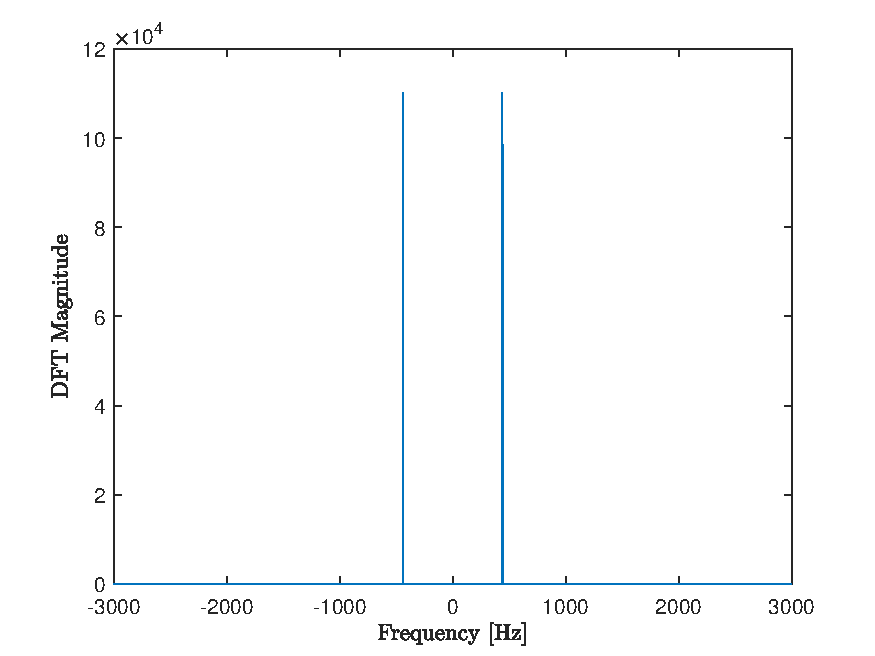
\includegraphics[width=\textwidth]{problem7_a440_pure_spectra.pdf}
    %     \caption{Low Dur}
    % \end{subfigure}
    \caption{Spectra and Harmonics of the Signals\vspace{-0.5cm}}
    \label{note_timbre_harmonics}
\end{figure}

Notice that the harmonics are present at multiple types and for diff frequencies.

\section{Creating Chirps}
Done.

\begin{figure}[ht]
    \centering
    \begin{subfigure}[b]{0.48\textwidth}
        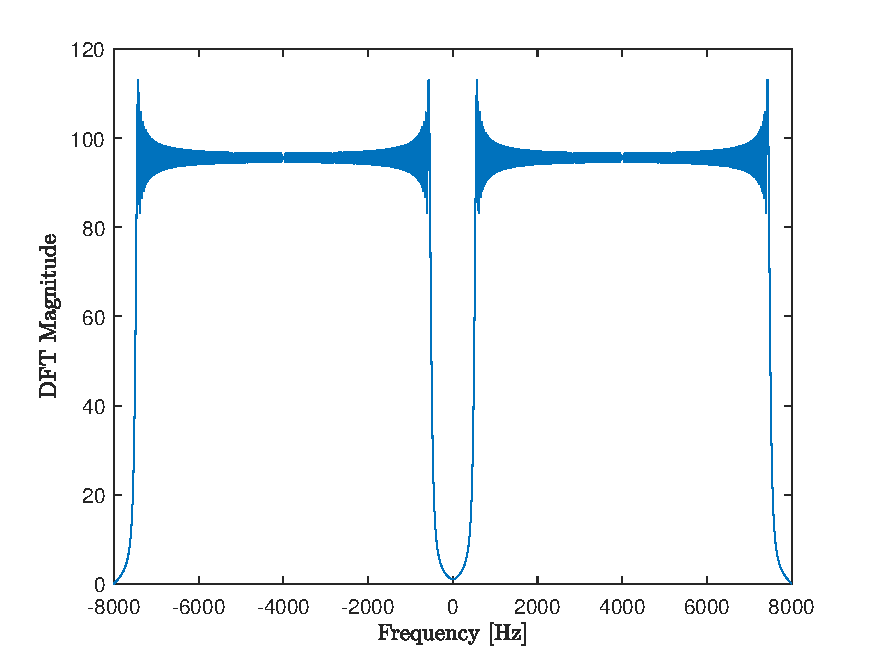
\includegraphics[width=\textwidth]{problem8_fft_linear_chirp.pdf}
        \caption{High Dur}
    \end{subfigure}
    \quad
    \begin{subfigure}[b]{0.48\textwidth}
        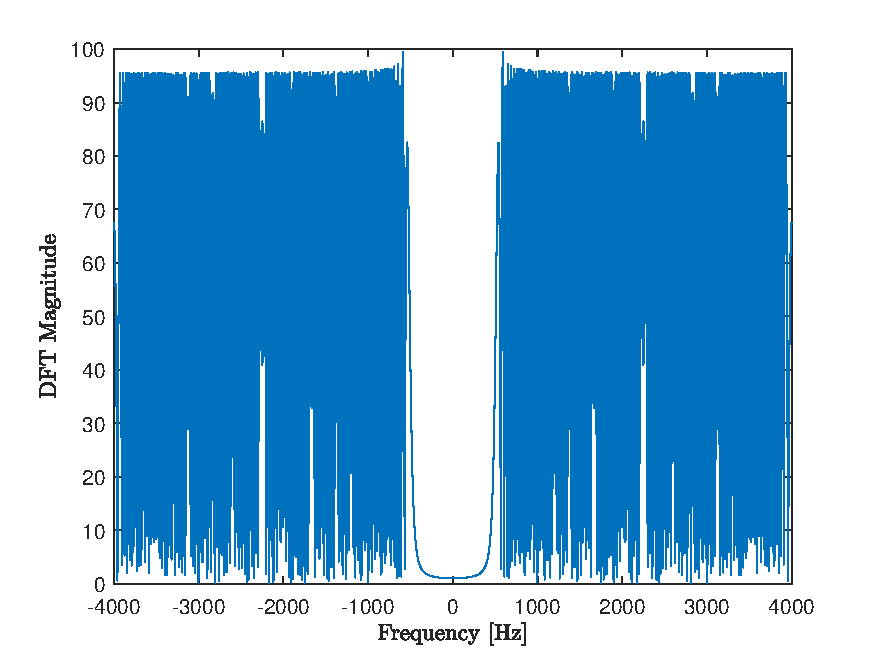
\includegraphics[width=\textwidth]{problem8_fft_subsampled_linear_chirp.pdf}
        \caption{Low Dur}
    \end{subfigure}
    \caption{Linear Chirps\vspace{-0.5cm}}
    \label{linear_chirp_fft}
\end{figure}

\section{Developing Simple Spectrograms}
Done. The spectrogram was made using rectangular windows with no overlaps. This causes spctral leakage, but since we have crafted a signal with exact frequencies and single tones at any given time, the spectrogram is very clear. Check figure xyz. In code, we call this manual construction function a \texttt{sonograph} as an alias, since the \texttt{spectrogram} function already exists in \textsc{MATLAB}.

\begin{figure}[ht]
    \centering
    \begin{subfigure}[b]{0.48\textwidth}
        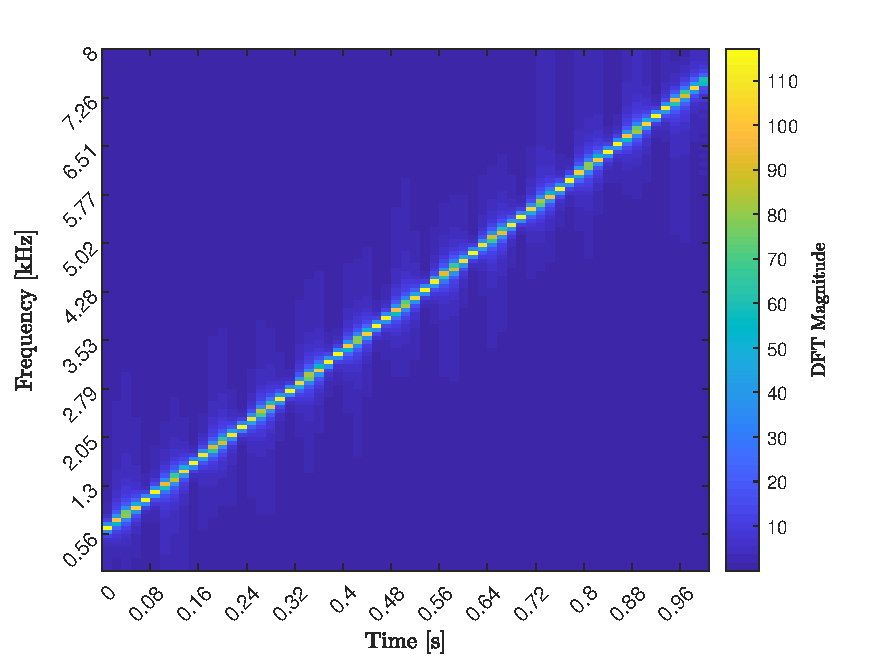
\includegraphics[width=\textwidth]{problem9_sonogram_linear_chirp.pdf}
        \caption{High Dur}
    \end{subfigure}
    \quad
    \begin{subfigure}[b]{0.48\textwidth}
        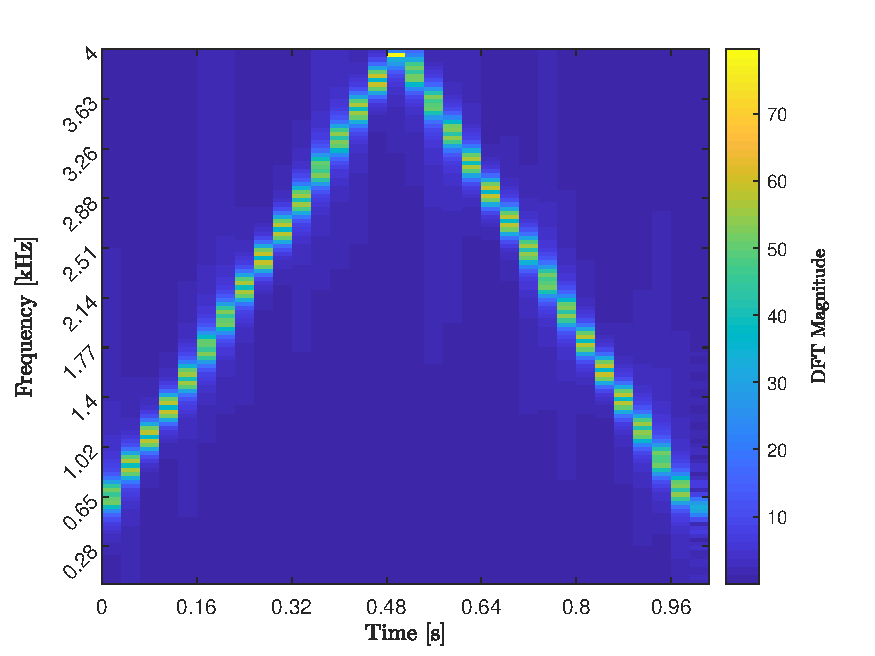
\includegraphics[width=\textwidth]{problem9_sonogram_subsampled_linear_chirp.pdf}
        \caption{Low Dur}
    \end{subfigure}
    \caption{Linear Chirps\vspace{-0.5cm}}
    \label{linear_chirp_spectrogram}
\end{figure}

\section{Doppler Effect and Tracking Chirps on Spectrograms}
Done. $f_0 = 6.7418e+03$, $v = 84.4658$, $d=40.4337$.

\begin{figure}[ht]
    \centering
    \begin{subfigure}[b]{0.48\textwidth}
        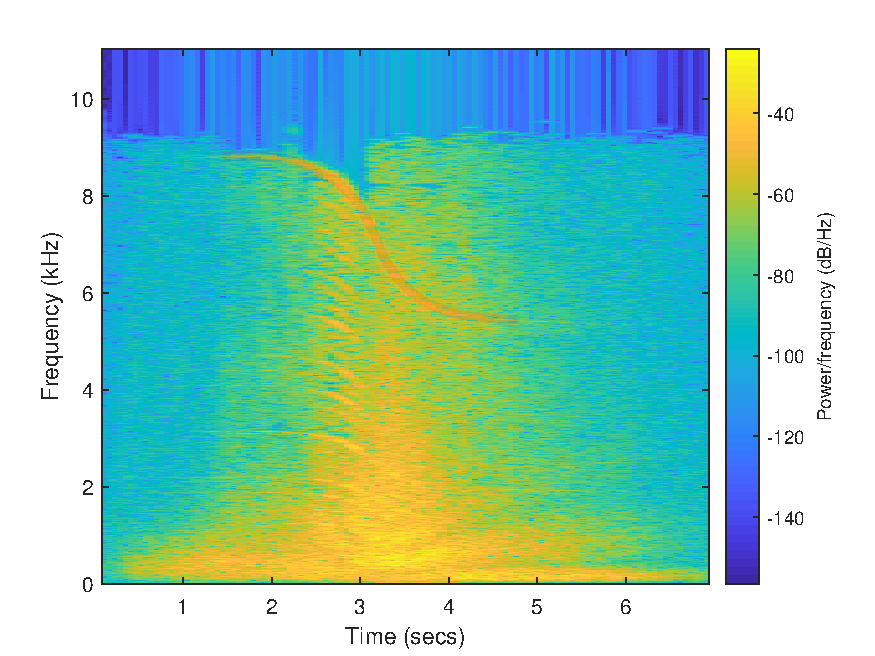
\includegraphics[width=\textwidth]{problem10_jet_spectrogram_doppler_shift_tracking.pdf}
        \caption{High Dur}
    \end{subfigure}
    \quad
    \begin{subfigure}[b]{0.48\textwidth}
        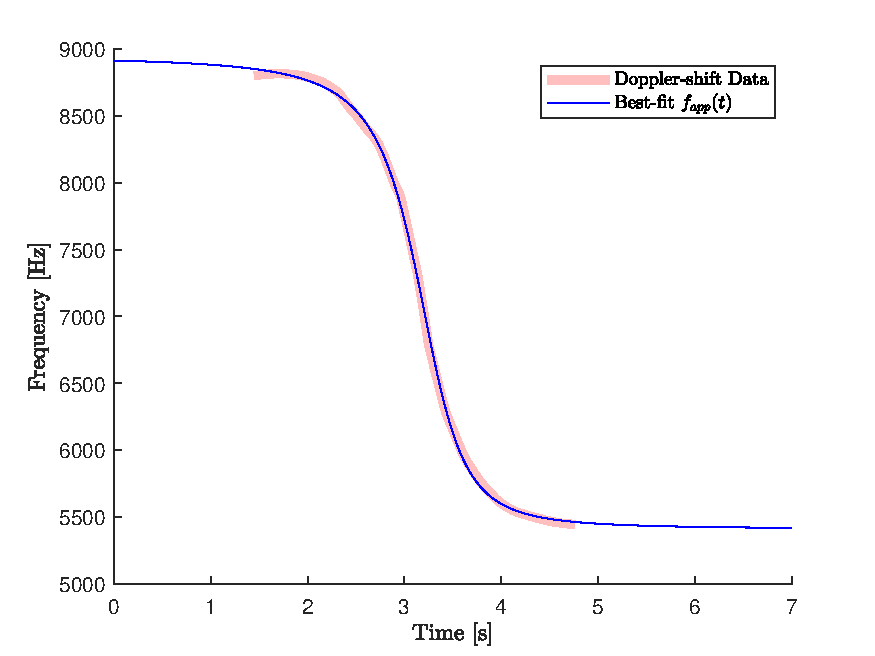
\includegraphics[width=\textwidth]{problem10_f_app_best_fit_estimate.pdf}
        \caption{Low Dur}
    \end{subfigure}
    \caption{Doppler Shift Tracking and Estimate\vspace{-0.5cm}}
    \label{doppler_shift_chirp}
\end{figure}

\section{Generating Random Noise}
Done. White: ; Pink: Low-frequency filtering of a white noise signal; Brown: Integration of a white noise signal. Give the procedure followed in code.

\begin{figure}[ht]
    \centering
    \begin{subfigure}[b]{0.31\textwidth}
        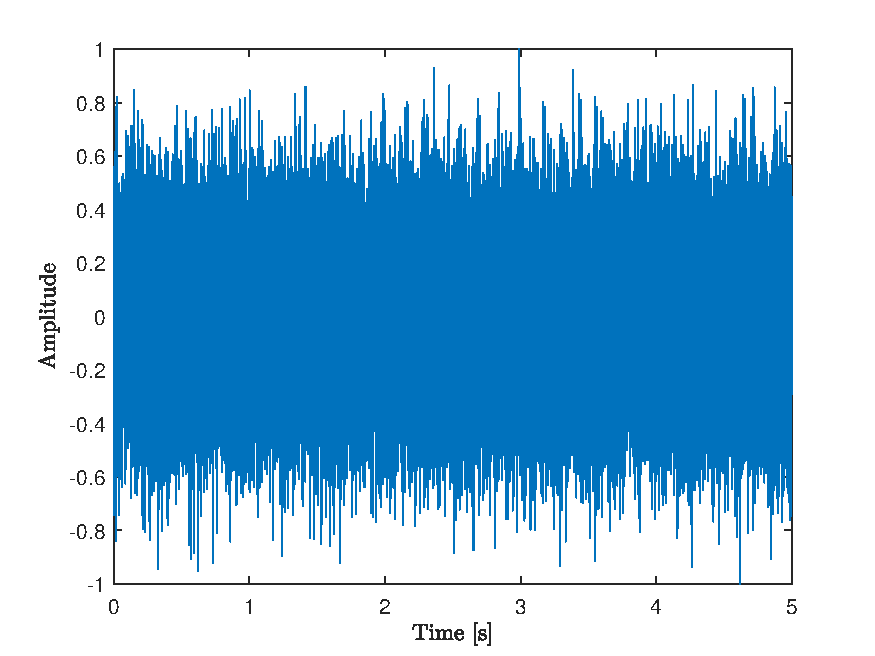
\includegraphics[width=\textwidth]{problem11_white_noise_time.pdf}
        \caption{High Dur}
    \end{subfigure}
    \quad
    \begin{subfigure}[b]{0.31\textwidth}
        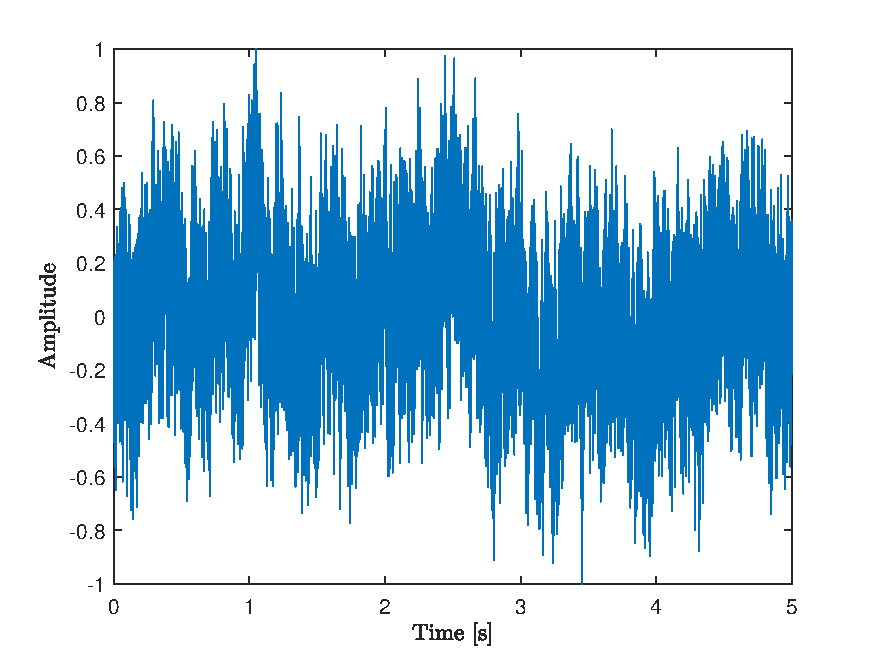
\includegraphics[width=\textwidth]{problem11_pink_noise_time.pdf}
        \caption{Low Dur}
    \end{subfigure}
    \quad
    \begin{subfigure}[b]{0.31\textwidth}
        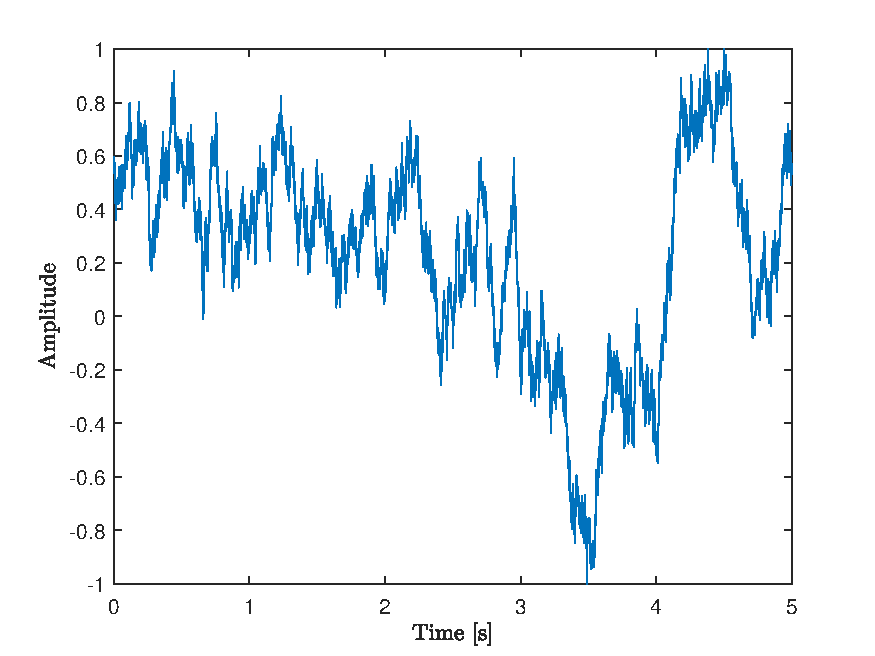
\includegraphics[width=\textwidth]{problem11_brown_noise_time.pdf}
        \caption{Low Dur}
    \end{subfigure}
    \caption{Color Noise in Time Domain\vspace{-0.5cm}}
    \label{color_noise_time_domain}
\end{figure}

\begin{figure}[ht]
    \centering
    \begin{subfigure}[b]{0.31\textwidth}
        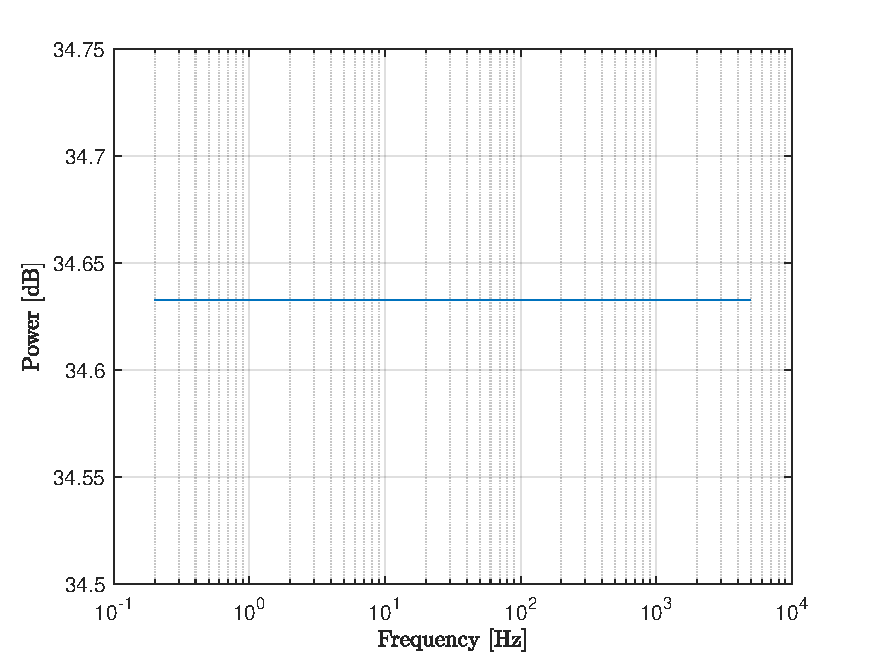
\includegraphics[width=\textwidth]{problem11_white_noise_power_spectrum_db.pdf}
        \caption{High Dur}
    \end{subfigure}
    \quad
    \begin{subfigure}[b]{0.31\textwidth}
        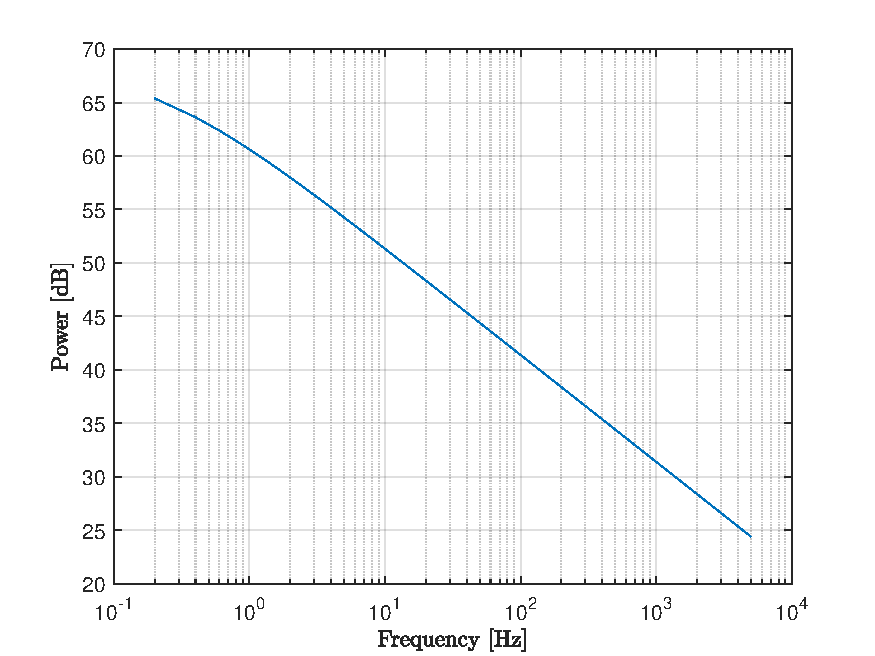
\includegraphics[width=\textwidth]{problem11_pink_noise_power_spectrum_db.pdf}
        \caption{Low Dur}
    \end{subfigure}
    \quad
    \begin{subfigure}[b]{0.31\textwidth}
        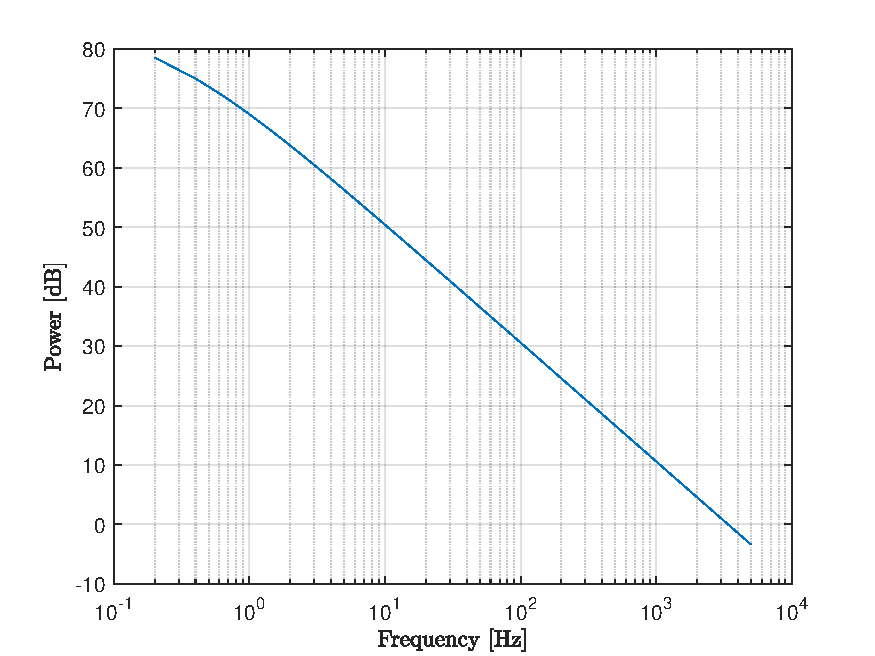
\includegraphics[width=\textwidth]{problem11_brown_noise_power_spectrum_db.pdf}
        \caption{Low Dur}
    \end{subfigure}
    \caption{Power Spectrum of Color Noise\vspace{-0.5cm}}
    \label{color_noise_freq_domain}
\end{figure}

\section{Simpler Generation of Uniform Random (White) Noise}
Done. For $U \sim \mathcal{U}(0,1)$ and $W$ to be uncorrelated uniform white noise signal in the PCM encoding, i.e. $W \in [-1,1]$, we can use the simple transform:
\[
    W = 2 U - 1
\]

Can be verified in the frequency domain. Time domain sequence given in \ref{uniform_white_noise}.

\begin{figure}[ht]
    \centering
    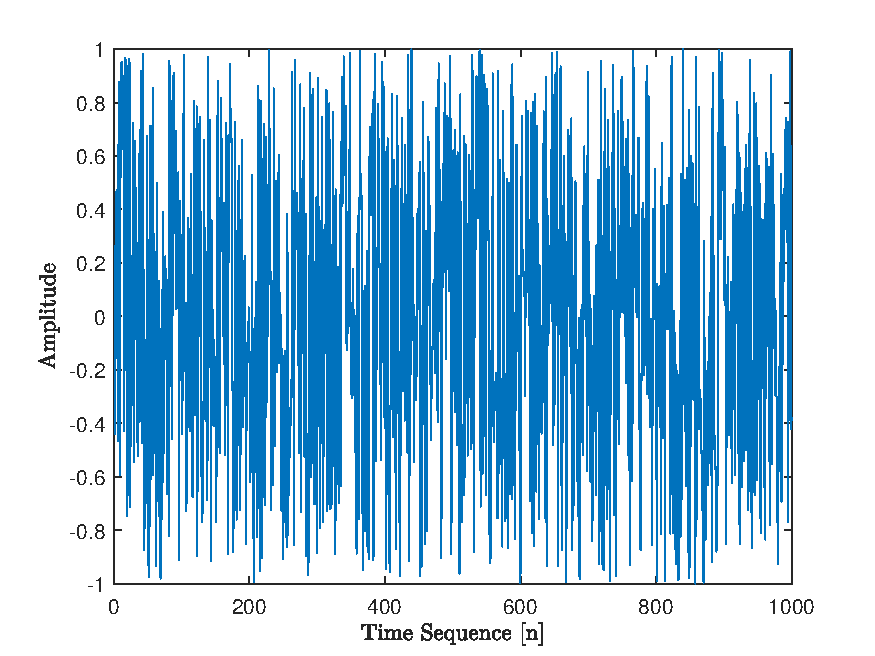
\includegraphics[width=0.5\textwidth]{problem12_uniform_white_noise_sequence.pdf}
    \caption{Uniform White Noise Sequence\vspace{-0.5cm}}
    \label{uniform_white_noise}
\end{figure}

\newpage
\clearpage
\section*{Appendix}

MATLAB code for prob 4, dialtone decode algorithm, goes here.

\begin{lstlisting}
% simple dtmf decode algorithm for a subset of tones (can be extended)
input_dtmf_tone = '';
[signal, Fs]    = audioread(input_dtmf_tone);

N   = length(signal);   % number of points in input signal and its fft
df  = Fs/N;             % frequency increment in nyquist range
fr  = -Fs/2:df:Fs/2-df; % frequency range (nyquist range)

fr_eps      = 10;         % frequency window around pure tones
dtmf_matrix = [1 2; 4 5]; % (partial) dtmf decode matrix; indexed by lower and upper band freqs
signal_fft  = fftshift(fft(signal)); % fft of the input signal

% get magnitude of each tone's contribution to the signal spectrum
m_fl1 = sum(2*abs(signal_fft(abs(fr - fl1) < fr_eps)));
m_fl2 = sum(2*abs(signal_fft(abs(fr - fl2) < fr_eps)));
m_fu1 = sum(2*abs(signal_fft(abs(fr - fu1) < fr_eps)));
m_fu2 = sum(2*abs(signal_fft(abs(fr - fu2) < fr_eps)));

% get dtmf decoding matrix indexes
[~, fl] = max([m_fl1 m_fl2]);
[~, fh] = max([m_fu1 m_fu2]);

dtmf_tone = dtmf_matrix(fl, fh); % algorithm output
\end{lstlisting}

\end{document}